For the task of classification, in which observations are globally known it is not necessary to model joint probability distribution over all possible outputs and observed values. Instead, a conditional distribution $P(y|x)$ is modelled, which represent a distribution of output variables on condition that input variables take an observed form. One of the methods that aim to to find the conditional distribution between variables is named Conditional Random Fields \cite{crf_lafferty}. This is a type of Markov Random Fields that can be viewed as undirected graphical models, which represent both observations, and output labels. With the use of factor graphs, factorisation of a probability distribution can be modelled. Then, those graphs contain two different types of variable nodes, inputs and outputs \cite{crf_sutton}. The first ones are observed input variables $x_i$, which are dependent on an application. For semantic image segmentation, $x_i$ would denote individual pixels from a single image $x$ taken from the set of all available images $X$. Input nodes are represented in terms of feature vectors containing observed properties of an individual image pixel expressed in a numerical form. A great advantage of Conditional Random Fields is that they can involve a large variety of different features. Input variable nodes are connected via factors to the second type of nodes, which are known as hidden nodes, as they cannot be directly obtained from an observed object. Those nodes represent a configuration of output variables denoted as $y$. For the task of semantic image segmentation, an output variable $y_i$ would represent a label assigned to a given pixel from a set of all possible labels $\pazocal{Y}$, and $y$ would represent a labelling for a whole image. Output nodes are as well connected with each other with the use of factors making it possible to take into consideration relations between neighbouring entities like pixels in an image. Figure \ref{fig:factor_graph_crf} presents how such a graph can be constructed on an example of an image with size $3\times3$ pixels.
\begin{figure}[ht]
    \centering
    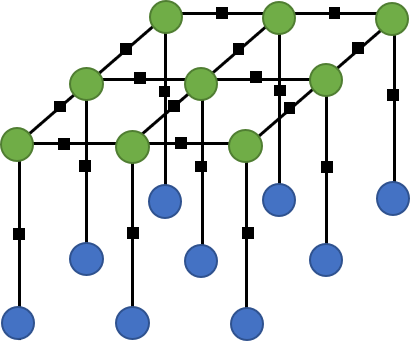
\includegraphics[width=0.5\textwidth]{structured_prediction/factor_graph_crf}
    \caption{Factor graph representing an image $3\times3$ pixels with input nodes marked in blue, and output nodes in green}
     \label{fig:factor_graph_crf}
\end{figure}

On the graph, blue circles represent input nodes with observed variables, and green circles a hidden layer of output nodes. Factors, which join each output node to the corresponding input node as well as every neighbouring output nodes are marked as black squares. Between each pair factor – node there is an edge presented as a line, which connects them. This is the simplest type of the graph with relations only between input and output nodes, and neighbouring output nodes. However, it is also possible to introduce other dependencies, for example between an output node and observation nodes related to neighbouring output nodes. For the sake of clearer explanation in following equations it will be assumed that there are relations between one input and one output node, and between two neighbouring output nodes only.

Conditional Random Fields model distribution $P(y|x)$ of a single labelling $y$ based on observed features of an image $x$. This distribution can be expressed in terms of energy as in formula \ref{eq:conditional_probability_energy}, with constant $Z$ computed as in equation \ref{eq:conditional_probability_z}.
\begin{align}
    \label{eq:conditional_probability_energy}
    P(y|x,w) &= \frac{1}{Z(x,w)} \exp{(-E(x,y,w))} \\
    Z(x,w) &= \sum_{y \in \pazocal{Y}}{\exp{(-E(x,y,w))}}
    \label{eq:conditional_probability_z}
\end{align}
Then, assuming an underling factor graph, energy of the whole system can be expressed as a summation of energies of individual factors, as it has already been presented in formula \ref{eq:joint_probability_distribution_factors}. However, for Conditional Random Fields a factor graph is composed of two types of nodes, input and output nodes. As a result, there are two sets of factors, a set $\pazocal{F}_1$ of factors between an output node and an input node, and a set $\pazocal{F}_2$ of factors between two neighbouring output nodes. Hence, the energy of the whole system can be expressed as two summations, one over the set of factors $\pazocal{F}_1$ and the second one over a set $\pazocal{F}_2$. As each factor $F \in \pazocal{F}_1$ is bound exactly to one input node and one output node the first summation over the set $\pazocal{F}_1$ may be expressed as a summation over all output nodes $i \in V$, which will compute energies for factors that are between the current output node an an input node assigned to it. Similarly, summation over factors from $\pazocal{F}_2$ is equivalent to summation over every pair of output nodes $i,j \in V$ that will compute energy for a factor that is between them. Hence, the formula for energy for a factor graph modelling Conditional Random Fields is presented in formula \ref{eq:energy_crf_intro}.
\begin{equation}
    \label{eq:energy_crf_intro}
    \begin{aligned}
        E(x,y,w) &= \sum_{F \in \pazocal{F}_1}E_F(x_F,y_F,w) + \sum_{F \in \pazocal{F}_2}E_F(y_F,w) \\
        &=\sum_{i\in V}{E_1}({y_i},{x_i},w) + \sum_{i,j \in V}{E_2}({y_i},{y_j},w)
    \end{aligned}
\end{equation}
Factor energy is defined differently depending on the factor type. Energy $E_1$ of factors $\pazocal{F}_1$ is called a unary potential. It models a relationship between observed features and a predicted label. It should assign high values of energy for a wrong label assigned to an output node of a given input node, and low energy values for proper assignments. It is used to promote a situation in which two nodes which are similar in terms of their feature vectors have the same label. Energy $E_2$ for factors from the set $\pazocal{F}_2$ is named a pairwise potential and it reflects a relation between labels of neighbouring output nodes. It introduces a penalty if neighbouring output nodes have a different label by assigning high energy values to such configurations, which as a result lower probability of their occurrence.
What is more, factor energy can be parametrised with a set of weights $w$, which can be obtained by a training process. Then, energy is dependent on three types of variables, inputs, outputs, and parameters \cite{inference_crf}, and can be expressed as . A more detailed explanation of energy function and its formulation will be provided in \textit{section \ref{sec:energy}: \nameref{sec:energy}}.

In order to make predictions about an unobserved object, it is necessary to find such a combination of output variables in a factor graph that will give the lowest energy as this would be a most probable setting. However, it is computationally intractable to calculate graph energy for every possible label configuration especially for problems involving large data structures. On an example of semantic image segmentation, even for a small problem of segmenting an image with size $100\times100$ pixels into two classes, it would require to calculate energy for $2^{100\times100}$ combinations and real-life problems are much more complicated. Because of this, in most cases, it is impossible to obtain an exact solution for classification problems based on factor graph energy. Though, it is possible to approximate a solution.